\section{Cost and Schedule}



%%%%%%%%%%%%%%%
\subsection{Costs}

The costs for the \dword{jpo} are still being compiled. These costs will first be presented to the DOE in the second half of August of 2019. After the data is submitted to the DOE the table in the \dword{tdr} will be updated.


\fixme{will come from Gina and be generated}


\subsection{Schedule}

The detector installation planning hinges on the date when the \dword{jpo} is permitted to begin work underground. According to the \dword{dune} \dword{cf} schedule the \dword{jpo} receives the \dword{aup} for  the north cavern and \dword{cuc} in \cucbenocc{}.  The  \dword{sdwf} will be in place approximately 6 months before the warm structure installation begins, i.e., in spring 2022. Building the schedule for the \dword{spmod} 1 Installation after \dword{aup} is a complicated dance that depends on many entities including \dword{cf}, \dword{lbnf}, and \dword{sdsta}.  The maximum number of people allowed underground is 144 which is the number of people that can be evacuated in one hour.  This places a hard bound on how much work can be perfored underground at any time and is particularly critical during the excavation of Cavern 3 when \dword{cf} is still active. Figure \ref{fig:Overview-of-SinglePhase-Schedule} shows the main activities for the \dword{detmodule} \#1 installation and  the high level milestones are shown in Table \ref{tab:sp-iic-sched}.

The cost, schedule, and labor estimates are based on two 10 hour shifts per day, 4 days a week. Work efficiency should be a maximum of 70 percent.  The cage ride, and shift meetings, lunch, coffee breaks, and gowning to go into the cleanroom takes up approximately 2-3 hours per day. Some low level of effort is planned on Friday, Saturday, and Sunday to monitor the \coldbox{}es and take data. 




%This is a standard table template for the TDR schedules.  It contains overall FD dates from Eric James as of March 2019 (orange) that are held in macros in the common/defs.tex file so that the TDR team can change them if needed. Please do not edit these lines! Please add your milestone dates to fit in with the overall FD schedule. 

\begin{dunetable}
[\dword{sp} Installation, Integration, and Commissioning Milestones]
{p{0.65\textwidth}p{0.25\textwidth}}
{tab:sp-iic-sched}
{\dword{sp} Installation, Integration, and Commissioning Schedule}   
Milestone & Date (Month YYYY)   \\ \toprowrule
Ash River phase 0 complete &  March 2020    \\ \colhline
Ash River phase 1 complete & June 2021     \\ \colhline
Installation Preliminary Design Review & August 2021     \\ \colhline
Ash River phase 2 complete &  July 2022    \\ \colhline
Installation Final Design Review  & September 2022     \\ \colhline
\rowcolor{dunepeach} Start of \dword{pdsp}-II installation& \startpduneiispinstall      \\ \colhline
\rowcolor{dunepeach} Start of \dword{pddp}-II installation& \startpduneiidpinstall      \\ \colhline
 \dword{cuc} \dword{prr} & July 2021     \\ \colhline
Installation \dword{prr} &  August 2022    \\ \colhline
\rowcolor{dunepeach}South Dakota Logistics Warehouse available& \sdlwavailable      \\ \colhline
Begin procurement of \dword{cuc} equipment  &   April 2022   \\ \colhline
Start production of installation infrastructure Detector \#1 & August 2022     \\ \colhline
\rowcolor{dunepeach}Beneficial occupancy of cavern 1 and \dword{cuc}& \cucbenocc      \\ \colhline
Start construction warm structure cryostat \#1   & October 2022     \\ \colhline
Start outfitting of \dword{cuc}  &  October 2022    \\ \colhline
\rowcolor{dunepeach} \dword{cuc} counting room accessible& \accesscuccountrm      \\ \colhline
Start installation of  cold structure Cryostat\#1 &  August 2023    \\ \colhline
Start installing Detector\#1 infrastructure  &  August 2023    \\ \colhline
\rowcolor{dunepeach}Top of \dword{detmodule} \#1 cryostat accessible& \accesstopfirstcryo      \\ \colhline
Begin Detector\#1 installation   &   June 2024   \\ \colhline

\rowcolor{dunepeach}Start of \dword{detmodule} \#1 TPC installation& \startfirsttpcinstall      \\ \colhline
\rowcolor{dunepeach}End of \dword{detmodule} \#1 TPC installation& \firsttpcinstallend      \\ \colhline
TCO detector \#1 closed  &  July 2025    \\ \colhline
\rowcolor{dunepeach}Top of \dword{detmodule} \#2 accessible& \accesstopsecondcryo      \\ \colhline
Start of cryogenic operation for detector \#1  &  August 2025    \\ \colhline
 \rowcolor{dunepeach}Start of \dword{detmodule} \#2 TPC installation& \startsecondtpcinstall      \\ \colhline
\rowcolor{dunepeach}End of \dword{detmodule} \#2 TPC installation& \secondtpcinstallend      \\ \colhline
Start of  detector\#1 commissioning  & January 2027     \\ \colhline                        \\
\end{dunetable}



\begin{dunefigure}[Overview of the single-phase schedule]
{fig:Overview-of-SinglePhase-Schedule}
{Schedule Overview of the Single Phase Detector \#1}                
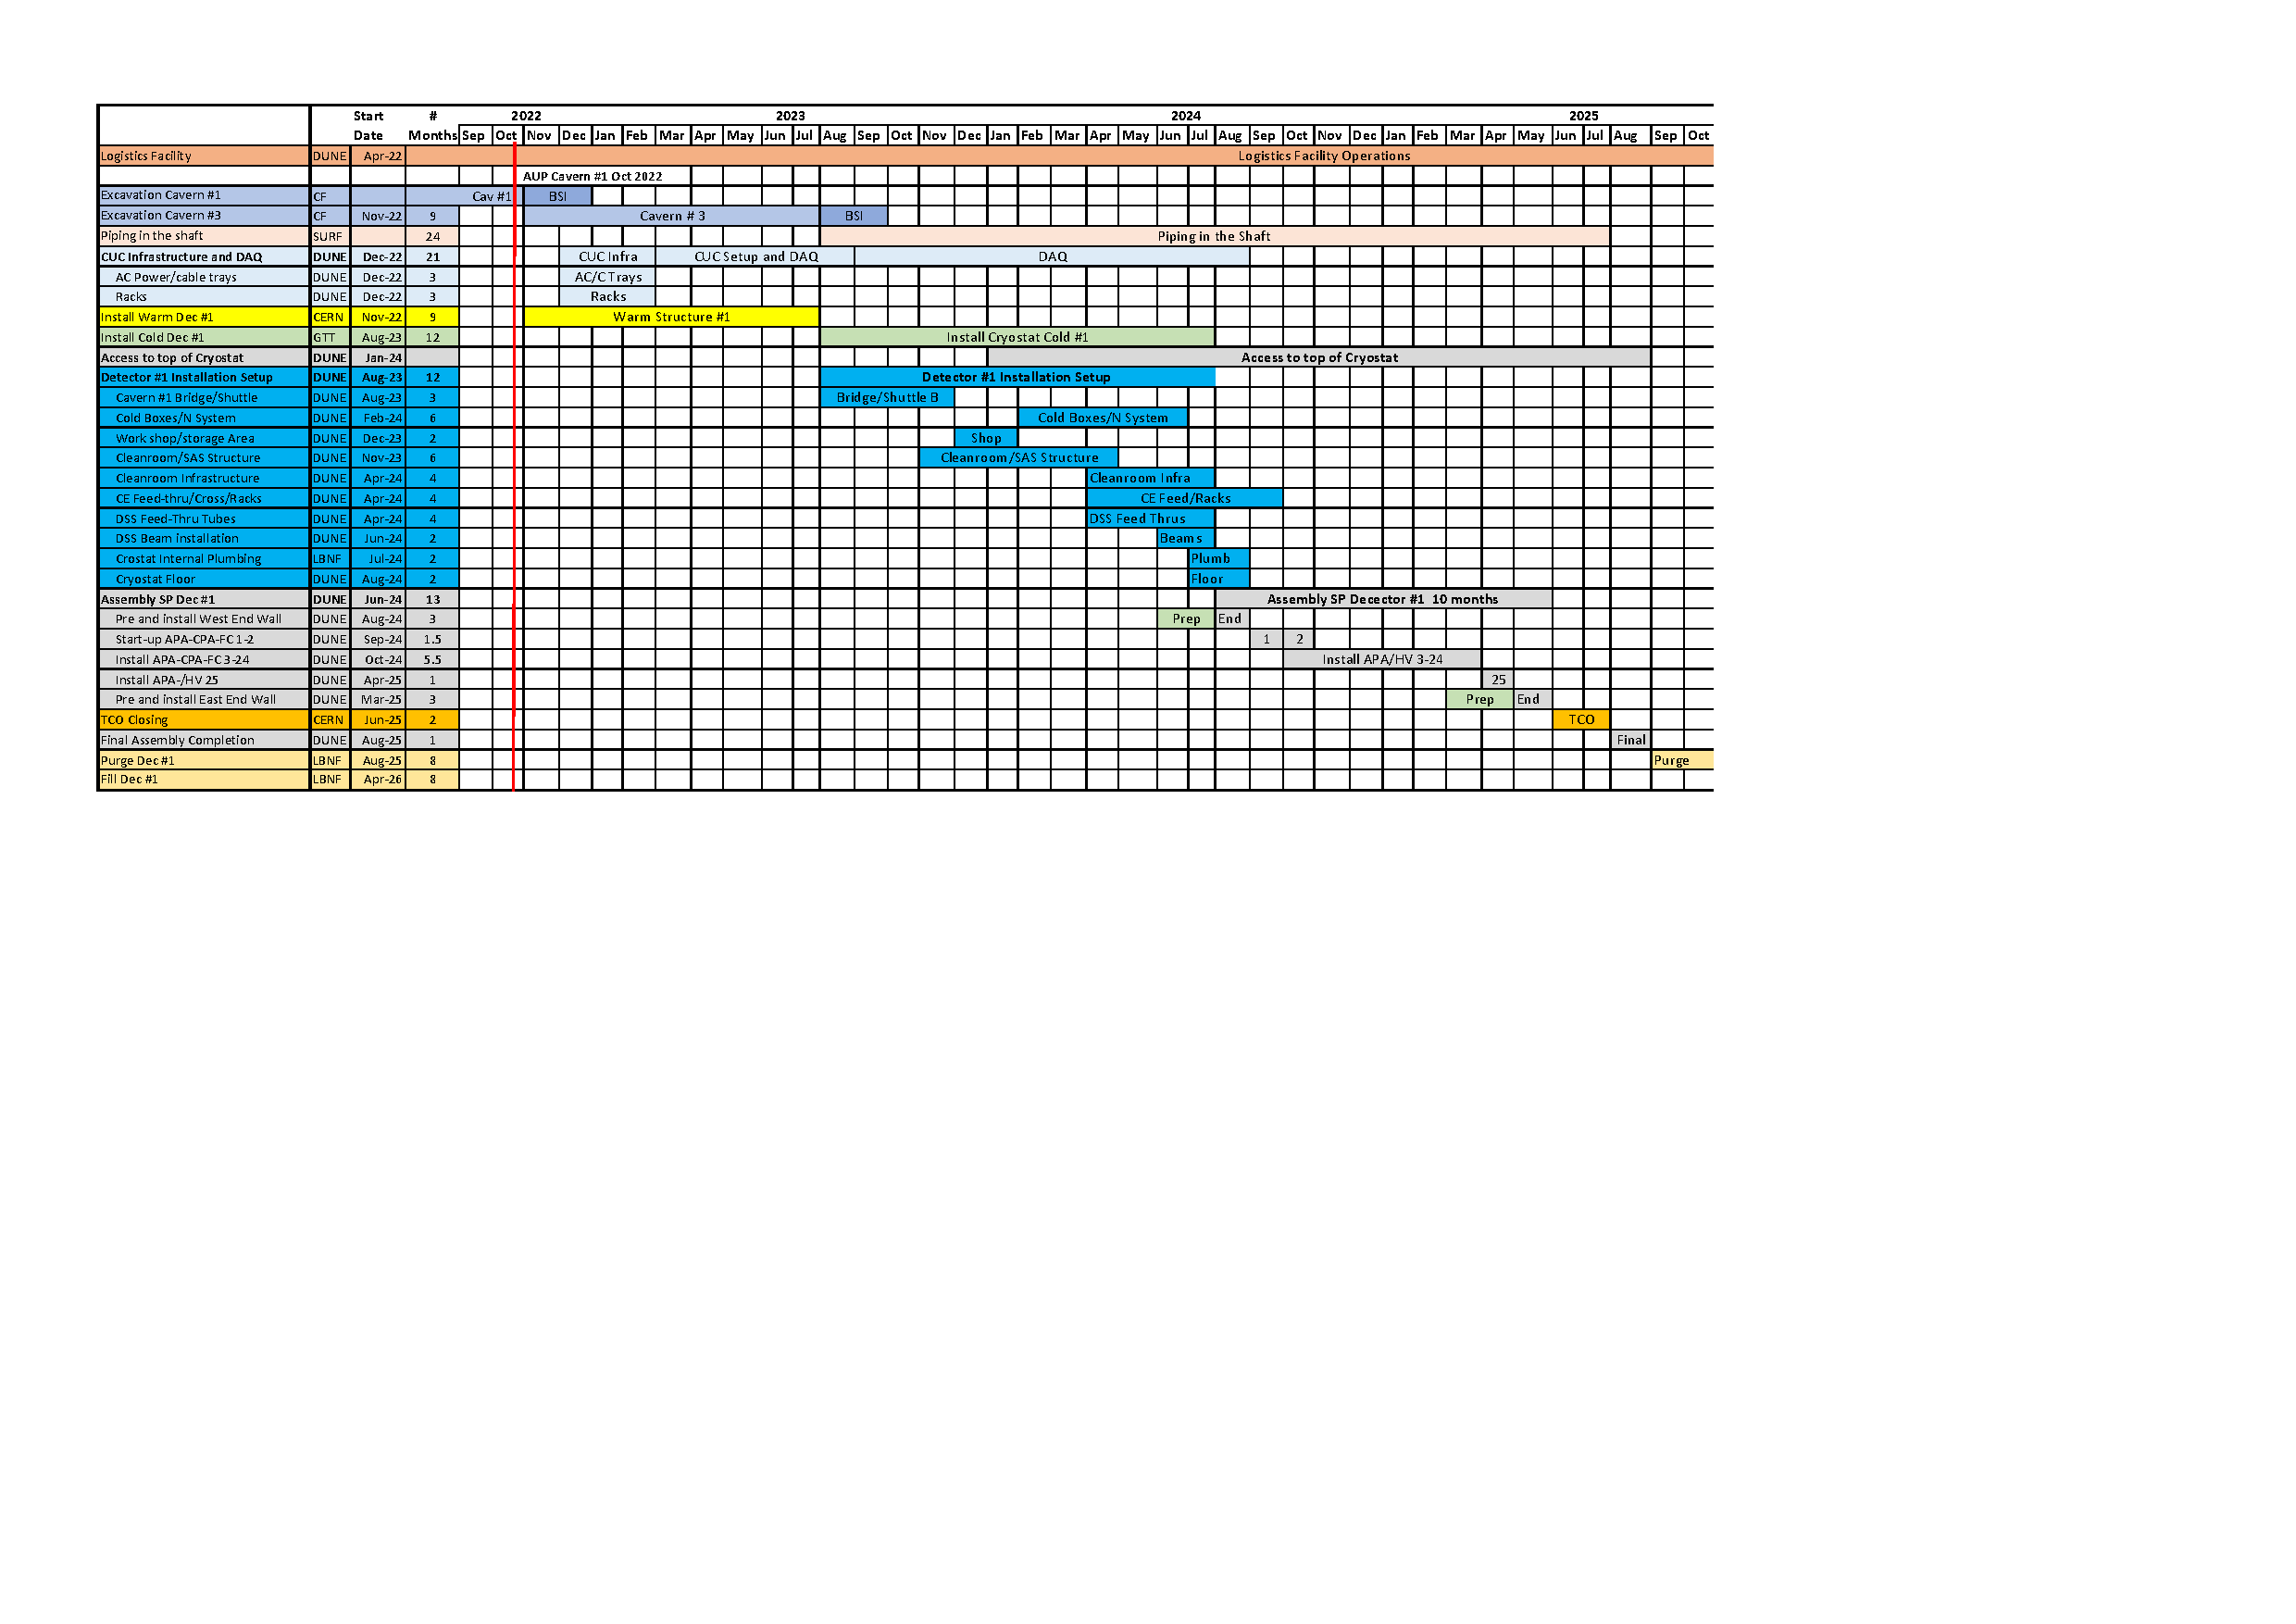
\includegraphics[width=0.98\textwidth]
{Overview-of-SinglePhase-Schedule}
\end{dunefigure}



As described earlier there are three basic schedule phases for Detector 1 installation:

\begin{itemize}
    \item {\bf \dword{cuc} Installation Phase:}
    This period, which is described in detail in section \ref{sec:fdsp-tc-inst-CUC}, can start once \dword{aup} has been received for the north cavern and the \dword{cuc}. This is also the same time that excavation of the south cavern and installation of the warm structure by \dword{lbnf} begins. As no more than 144 \dwords{fte} will be allowed underground at a time,  access to the underground area will be minimal during this period for \dword{dune} personnel.  Work in this period is limited to work inside the \dword{cuc} and surface dataroom. Installing the basic rack infrastructure in the datarooms will take an estimated three months, and then installation and testing of the \dword{daq} will continue over the next 12 month period. The \dword{daq} is needed at the start of detector installation.  
    
    \item {\bf Installation Setup Phase:} This phase,  described in detail in section \ref{sec:fdsp-tc-inst-setup}, is when the majority of the infrastructure is installed. 
    This is a critical training period, so getting lead-workers, riggers, and equipment operators familiar with the tasks is a priority, and adjusting crews to ensure balanced teams.  
    Before this phase, the \dword{dune} trial assembly equipment at Ash River will be used to begin the training process. This is a more difficult phase to schedule and may require frequent adjustment, with multiple projects going forward at once.
    Immediately after the cryostat warm structure is complete the north-south bridge is constructed. Following this the bridge crane under the bridge can be installed. A few months after the cryostat warm structure is complete the \dword{cf} work is also complete and the 80 of 144 underground workers which \dword{cf} had been using are available to the \dword{jpo}, working two 10 hour shifts per day begins, and the \dword{uit} team doubles in size.  Peripheral work on the cleanroom structure and assembly towers can then begin as they will not take up too much floor space. Once the  cryostat cold structure is approximately six months into the installation schedule most of the foam has been installed and floor space becomes available in the north cavern. The \coldbox construction must begin immediately at this point because the welding takes approximately six months. In parallel, the machine shop area can be set up. As the membrane installation nears completion the walls of the cleanroom can be installed and the remaining equipment. 
    
    Installation of the \dword{dss} could begin during the final installation stages of the cryostat cold structure because they both require full-height scaffolding for the welding on the top of the cryostat. The \dword{protodune} \dword{dss} was installed this way. This requires a crew on top of the cryostat installing the \dword{dss} support feedhroughs from the top, as shown in Figure~\ref{fig:install-dss-feedthru}.  The details have not yet been worked out with the contractor, so work may be done in stages. 

    
    \item {\bf Detector Installation Phase:} The final detector installation phase begins with an operational readiness review to check that all documentation and procedures are in place. After the east endwalls are installed, a start-up period of 1.5 months begins for the first two rows of \dword{tpc} components.  To meet this schedule, three assembly lines, three coldboxes, and separate crews in the cryostat, all working in parallel are needed.  It will take 5.5 months to install rows 3-24 and about 1 month for row 25. Closing the \dword{tco} will take approximately two months for the cryostat cold structure contractor. During this time, there is no access to the cryostat.  Once this is completed, the final instrumentation is completed, and the purge can begin. 
    
\end{itemize}



  




% clear the figure buffer before starting the next section
%\clearpage


\subsection{Detector Commissioning Phase}
\label{sec:fdsp-tc-inst-comiss}

After the \dword{spmod} is installed in the cryostat, much work remains before it can be operated. 
The cryostat manufacturer must come back to close the \dword{tco}. 
First they install the missing steel panel which completes the cryostat's outer structural hull. 
Then the remaining foam blocks and membrane panels which were stored inside the cryostat are installed. 
In this period personnel access is through the roof's access portholes. 



In parallel, the \lar pumps are installed at the ends of the cryostat and final connections are made to the recirculation plant. Next, everything is leak tested, and the cryogenics plant can be brought into operation. The system first purges the air inside the cryostat  by injecting pure \dword{gar} at the bottom  at a rate that fills the cryostat volume uniformly but faster than the diffusion rate. This ``piston purge'' process produces a column of \dword{gar}  that rises through the volume and pushes out the air.  When the piston purge is complete, misting nozzles inject a liquid-gas mix into the cryostat that cools the detector components at a controlled rate. 


Once the detector is cold, the filling process begins. \dword{lar} stored at the surface  at \dword{surf} is vaporized, brought down the shaft in gaseous form, and re-condensed underground. The \lar then flows through filters to remove any H$_2$O and O$_2$ before entering the cryostat. Given the volume of the cryostat and the limited cooling power for recondensing, \num{12} months will be required to fill the first \dword{detmodule}. The detector readout electronics will be on monitoring the status of the detector. 

Testing and constant monitoring of the detector will take place from \dword{tco} closing until the end of the filling process. 
Before the last access port is sealed:
\begin{enumerate}

    \item A pedestal and \dword{rms} characterization of all cold electronic channels will verify that all \dword{apa} front-end boards are responding and no dead channel or new noise sources arose following the \dword{tco} closing.
    
    \item A noise scan of all \dword{pd} channels is performed as last check before sealing.

    \item Each \dword{apa} wireplane will be checked to verify it is isolated from the \dword{apa} frame and properly connected to its \dword{hv} power supply through the following steps:
    
\begin{itemize}

    \item The \dword{shv} connector of each wireplane bias channel will be unplugged at the power supply, and both the resistance and capacitance between inner conductor and ground will be measured. 
    The resistance should show the wireplane is electrically isolated from the ground, while the capacitance value should match that of the cold \dword{hv} cable and the capacitance of the circuit on the \dword{apa} top frame.

    \item \SI{50}{V} is applied to each wireplane and the current drawn checked against the expected value.
    
    \item Nominal voltages are applied to each wireplane, and the current drawn is checked against the expected value. 
    
\end{itemize}

    \item A low \dword{hv} (i.e., \SIrange{1}{2}{kV}) is applied to the cathode, and the current drawn is checked against the expected value to ensure the integrity of the \dword{hv} line.

\end{enumerate}

During the piston purge process periodic monitoring of \dword{apa}, \dword{ce}, and \dword{pd} system noise (pedestal, \dword{rms}) will occur.

A number of the following tests, in addition to new ones, will instead take place during the cool-down phase:

\begin{enumerate}


    \item Each \dword{apa} wireplane isolation and proper connection to its \dword{hv} power supply will be checked at regular time intervals as was done before sealing the cryostat.
    
    \item \SIrange{1}{2}{kV} will be held on the cathode, and the current drawn will be  monitored constantly to observe the trend in temperature of the total resistance.
    
    \item \dword{ce} noise figures (pedestal, \dword{rms}) will be measured at regular intervals and their trends with temperature recorded.
    
    \item \dword{pd} system noise (pedestal, \dword{rms}) will be measured at regular intervals and its trend with temperature recorded.
    
     \item Values of the temperature sensors deployed in several parts of the cryostat will be monitored constantly to watch the progress of the cool down phase and to relate the temperature to the behavior of the other \dword{spmod} subsystems. 
     
\end{enumerate}

Regular monitoring of \dword{ce} and \dword{pd} noise, as well as checks of wireplane isolation and proper connections to the bias supply system will continue throughout the filling, recording noise variations as a function of the progressively reduced temperature. In addition,

\begin{enumerate}

    \item As each purity monitor is submerged in liquid, it will be turned on every eight hours to control \dword{lar} purity.
    
    \item As soon as top ground planes are submerged, \dword{hv} on the cathode will be raised up to \SI{10}{V} to check that the current drawn by the system agrees with expectations.

\end{enumerate}

Once the \dword{detmodule} is full, the drift \dword{hv} will be carefully ramped up following these steps:

\begin{enumerate}

    \item The need for a filter regeneration is evaluated before starting any operation;

    \item Once filter regeneration is completed (if needed), the \dword{lar} surface is examined using cameras to verify that the surface is flat, with no bubbles or turbulence;
    
    \item \dword{lar} recirculation is started, and \dword{lar} surface is examined again to see if activating the recirculation system introduced any turbulence into the liquid;
    
    \item Wait one day after beginning  recirculation to stabilize the \dword{lar} flow inside the \dword{detmodule}, then start the \dword{hv} ramp up.
    
\end{enumerate}

Cathode voltage is raised in steps over three days. 
On the first day, cathode voltage is first raised to \SI{60}{kV}, then to \SI{90}{kV} after waiting two hours, and finally to \SI{120}{kV} after waiting another two hours, and then left at this value overnight.
On the second day, cathode voltage is first raised to \SI{140}{kV}, then to \SI{160}{kV} after waiting four hours, and then left at this value overnight. 
On the third day, cathode voltage is first raised to \SI{170}{kV} and then to the nominal operating voltage of \SI{180}{kV} after waiting four hours. 
During each \dword{hv} ramp up, all \dword{ce} current draws are monitored, and the procedure is stopped if any of the current draws go out of the allowed range. 
During each waiting period, regular \dword{daq} runs monitor \dword{ce} and \dword{pd} noise and response, while cathode \dword{hv} and current draw stability are constantly monitored.

In \dword{pdsp}, this process took three days, after which the system was  ready for data-taking. With a detector twenty times larger, the process will take longer, but the turn on time should still be relatively short. 

